\begin{figure}[t]
\centering
\subfigure[$K=1$]{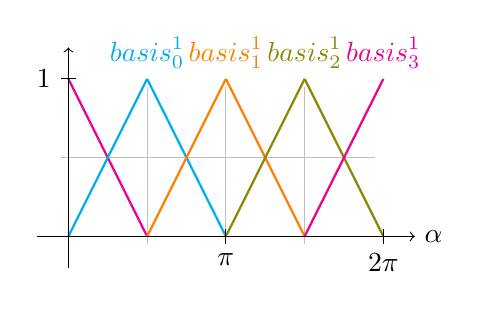
\begin{tikzpicture}
  \draw[color=lightgray] (-0.1, -0.1) grid (3.9, 1.9);

  \draw[thick,color=magenta] (0, 2) -- (1, 0);
  \draw[thick,color=cyan] (0, 0) -- (1, 2) node[above] {$\gls{basis}_0^1$};
  \draw[thick,color=cyan] (1, 2) -- (2, 0);
  \draw[thick,color=orange] (1, 0) -- (2, 2) node[above] {$\gls{basis}_1^1$};
  \draw[thick,color=orange] (2, 2) -- (3, 0);
  \draw[thick,color=olive] (2, 0) -- (3, 2) node[above] {$\gls{basis}_2^1$};
  \draw[thick,color=olive] (3, 2) -- (4, 0);
  \draw[thick,color=magenta] (3, 0) -- (4, 2) node[above] {$\gls{basis}_3^1$};

  \draw[->] (-0.4, 0) -- (4.4, 0) node[right] {$\alpha$};
  \draw[->] (0, -0.4) -- (0, 2.4);
  \draw (0.1, 2) -- (-0.1, 2) node[left] {$1$};
  \draw (2, 0.1) -- (2, -0.1) node[below] {$\pi$};
  \draw (4, 0.1) -- (4, -0.1) node[below] {$2\pi$};

\end{tikzpicture}
}
\hspace{1cm}
\subfigure[$K=2$]{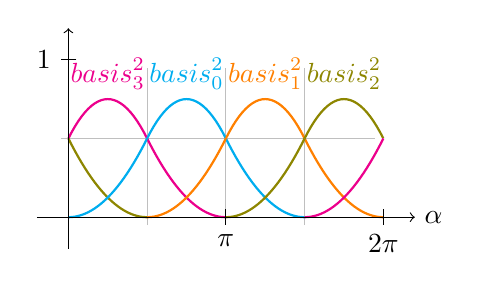
\begin{tikzpicture}
  \draw[color=lightgray] (-0.1, -0.1) grid (3.9, 1.9);

  \draw[color=cyan] (1.5,1.5) node[above] {$\gls{basis}_0^2$};
  \draw[color=orange] (2.5,1.5) node[above] {$\gls{basis}_1^2$};
  \draw[color=olive] (3.5,1.5) node[above] {$\gls{basis}_2^2$};
  \draw[color=magenta] (0.5,1.5) node[above] {$\gls{basis}_3^2$};

  \draw [thick,color=magenta,domain=0:1] plot (\x,(-2*\x^2+2*\x+1);
  \draw [thick,color=magenta,domain=1:2] plot (\x,(\x^2-4*\x+4);

  \draw [thick,color=olive,domain=0:1] plot (\x,(\x^2-2*\x+1);

  \draw [thick,color=cyan,domain=0:1] plot (\x,\x^2);
  \draw [thick,color=cyan,domain=1:2] plot (\x,-2*\x^2+6*\x-3);
  \draw [thick,color=cyan,domain=2:3] plot (\x,\x^2-6*\x+9);

  \draw [thick,color=orange,domain=1:2] plot (\x,(\x^2-2*\x+1);
  \draw [thick,color=orange,domain=2:3] plot (\x,(-2*\x^2+10*\x-11);
  \draw [thick,color=orange,domain=3:4] plot (\x,(\x^2-8*\x+16);

  \draw [thick,color=olive,domain=2:3] plot (\x,(\x^2-4*\x+4);
  \draw [thick,color=olive,domain=3:4] plot (\x,(-2*\x^2+14*\x-23);

  \draw [thick,color=magenta,domain=3:4] plot (\x,(\x^2-6*\x+9);

  \draw[->] (-0.4, 0) -- (4.4, 0) node[right] {$\alpha$};
  \draw[->] (0, -0.4) -- (0, 2.4);
  \draw (0.1, 2) -- (-0.1, 2) node[left] {$1$};
  \draw (2, 0.1) -- (2, -0.1) node[below] {$\pi$};
  \draw (4, 0.1) -- (4, -0.1) node[below] {$2\pi$};
\end{tikzpicture}
}
\caption[Geschlossene B-Spline-Funktionen]{Illustration geschlossener B-Spline-Funktionen $\gls{basis}_p^K \colon \left(0, 2\pi\right] \to \left[0, 1\right]$ für $P=4$ gleichmäßig verteilter Kontrollpunkte, einmal mit lokaler Kontrollierbarkeit $K=1$ (a) und einmal mit $K=2$ (b).}
\label{fig:bspline}
\end{figure}
